\documentclass[a4paper, french]{article}
\usepackage{config}
\author{Vincent Commin \& Louis Leenart}
\date{\today}
\setcounter{secnumdepth}{6}
\begin{document}

\begin{titlepage}
    \begin{flushleft}
        \includegraphics[width=5cm]{UL.jpg}\par
        \centering

        \vspace{13\baselineskip}
        \HRule \\[0.4cm]

        {\Huge
        GIF-4104 - TP 4\par}
        \vspace{0.4cm}
        \HRule
        \vfill
        Équipe 1 : Vincent Commin \& Louis Leenart\medskip \par
    \end{flushleft}
\end{titlepage}

\newpage
\section{Introduction}

Pour ce quatrième TP, nous avons implémenté la parallélisation d'inversion d'une matrice en utilisant
méthode de \href{https://fr.wikipedia.org/wiki/%C3%89limination_de_Gauss-Jordan}{\textit{\underline{Gauss Jordan}}}
avec  \href{https://www.khronos.org/opencl/}{\textit{\underline{OpenCL}}} et \href{https://www.openacc.org/}{\textit{\underline{OpenACC}}}. En se basant sur l'implémentation séquentielle proposée, nous avons suivi l'approche par réduction puis diffusion successives.

\section{Notre approche}

\subsection{OpenCL}

Dans ce TP, nous avons découvert l'utilisation d'OpenCL ainsi que ses particularités. En implémentant l'algorithme d'inversion de matrix de Gauss Jordan pour une architecture de GPU, nous avions en tête de diminuer le temps de calcul pour qu'il soit inférieur à celui obtenu avec l'utilisation uniquement du CPU.

L'algorithme que nous avons mis en place est le suivant :

\begin{lstlisting}[style=txt]
AI : Matrix [A I] // Shared amoung every GPU threads
Buffer : value array // Shared amoung every GPU
size, rank : integer

FOR k = 0 TO AI.rows DO
    max = 0, pivotIndex = k
    FOR i = k TO AI.rows DO // Find greatest pivot for column k
        IF (i mod size) == rank && abs(AI[i, k]) > max DO
            max = abs(AI[i, k]); pivotIndex = i
        DONE
    DONE

    Buffer[pivotIndex] = max
    pivotIndex = Reduce(MAX_LOG, Buffer) // Location of max value in Buffer

    IF IA[pivotIndex, k] == 0 DO throw exception DONE

    v = AI[k, k] // Normalisation
    FOR j = 0 TO AI.cols DO
        AI[k, j] = AI[k, j] / v
    DONE

    FOR i = 0 TO AI.rows DO // For each rows
        IF i mod size == rank && i != k DO
            AI[i] -= AI[k] * AI[i, k]
        DONE
    DONE
DONE

FOR i = 0 TO AI.rows DO // Copy right side of AI into result
    A = AI.getData()[slice(i * AI.cols + AI.rows, AI.rows, 1)]
DONE
\end{lstlisting}

L'utilisation que nous avons fait d'OpenCL est assez naïve : découvrant le langage, nous avons simplement essayé d'appliquer l'algorithme d'inversion. Pas encore suffisament familier avec les tenants et aboutissants de chacun des paramètres OpenCL, nous avons eu du mal à paramétrer ce dernier pour maximiser les performances. Nous avons par ailleurs remarqué que pour une taille de workgroup plus grande que 128, des erreurs de calculs ont commencé à appaitre, mais nous avons pas réussi à identifier la source de ce problème, c'est pourquoi nous conduirons nos calculs pour des matrix de taille maximum 128 x 128.

D'après les spécifications de la carte graphique utilisée, nous avons décidé d'utiliser un worker group de la taille de la matrice, et donc d'associer une ligne à chacun des worker, ce qui nous a permi d'obtenir les meilleurs résultats. La minimisation de l'accès à la mémoire globale n'a pu être notre priorité, et l'on remarque effectivement que chaque worker accède régulièrement à la mémoire globale ce qui n'est pas obtimal.

\subsection{OpenACC}

% TODO(Vincent)

\section{Machine utilisée pour les tests de performance}

\begin{center}
    \begin{tabularx}{0.6\textwidth}{|>{\raggedleft\arraybackslash}X|>{\raggedright\arraybackslash}X|}
        \hline
        Modèle & intel i7-8550U \\
        \hline
        Architecture & x86\_64 \\
        \hline
        OS & Archlinux \\
        \hline
        Fréquence CPU & 3.4GHz \\
        \hline
        C\oe urs (physique / logique) & 4 / 8 \\
        \hline
        Ram & 16 Go, 2400 $MT/s$ \\
        \hline
        GPU & Intel(R) UHD Graphics 620 \\
        \hline
        OpenCL & version 3.0 \\
        \hline
        GCC & version 11.2.0 \\
        \hline
        nvc++ & version 22.1 \\
        \hline
    \end{tabularx}
\end{center}

\section{Résultats obtenus}

\begin{center}
    \begin{tabularx}{\textwidth}{c c}
        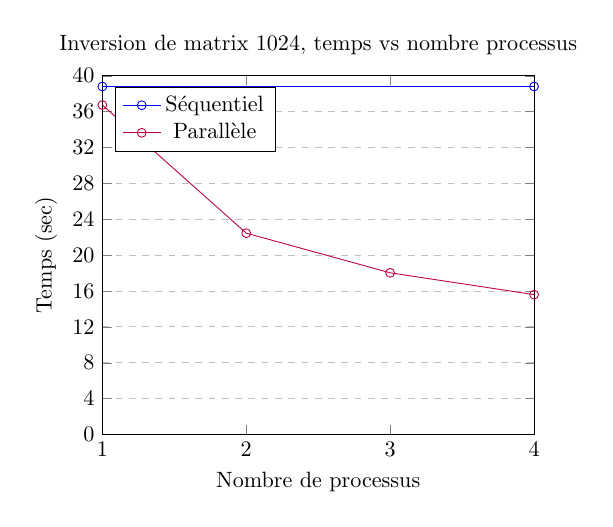
\begin{tikzpicture}[scale=0.8, transform shape]
            \begin{axis}[
                title={Inversion de matrix 1024, temps vs nombre processus},
                xlabel={Nombre de processus},
                ylabel={Temps (sec)},
                xmin=1, xmax=4,
                ymin=0, ymax=40,
                xtick={1, 2, 3, 4},
                ytick={0, 4, 8, 12, 16, 20, 24, 28, 32, 36, 40},
                legend pos=north west,
                ymajorgrids=true,
                grid style=dashed,
                ]
                \addplot[color=blue, mark=o] coordinates {(1, 38.8119)(4, 38.8119)};
                \addplot[color=purple, mark=o] coordinates {(1, 36.7437)(2, 22.4539)(3, 18.0343)(4, 15.5994)};

                \legend{Séquentiel, Parallèle}
            \end{axis}
        \end{tikzpicture}
        &
        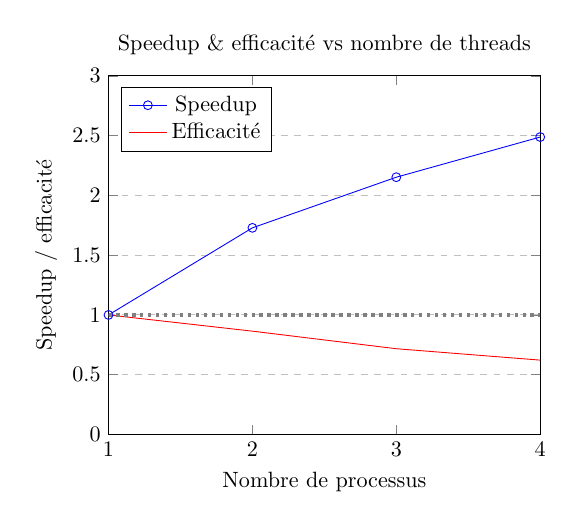
\begin{tikzpicture}[scale=0.8, transform shape]
            \begin{axis}[
                title={Speedup \& efficacité vs nombre de threads},
                xlabel={Nombre de processus},
                ylabel={Speedup / efficacité},
                xmin=1, xmax=4,
                ymin=0, ymax=3,
                xtick={1,2,3,4},
                ytick={0, 0.5, 1, 1.5, 2, 2.5, 3},
                legend pos=north west,
                ymajorgrids=true,
                grid style=dashed,
                ]
                \addplot[color=blue, mark=o] coordinates {(1, 1)(2, 1.728514868)(3, 2.152115691)(4, 2.488038001)};
                \addplot[color=red, mark=] coordinates {(1, 1)(2, 0.8642574341)(3, 0.7173718969)(4, 0.6220095004)};
                \addplot[color=gray, dotted, ultra thick] coordinates {(0, 1)(8, 1)};
                \legend{Speedup, Efficacité}
            \end{axis}
        \end{tikzpicture}
    \end{tabularx}
\end{center}

\newpage

\section{Analyse}


\section{Conclusion}

\end{document}